\chapter{Introduction}
\label{chap:introduction}
\section{Motivation} 
\label{sec:motivation}
Modern markets have, to a large extend, become computerized technological systems. Opportunistic investors and market makers likewise interact within these high-frequency marketplaces with the use of electronic algorithms. While generally aiming for (large) profits, the typical portfolio manager diversifies the available capital in a variety of assets simultaneously in order to reduce risk. \emph{Technical analysis}, which is the analysis of past stock prices, and \emph{fundamental analysis}, which is the analysis of a companies intrinsic value, are used to estimate weather individual assets are currently under- or overvalued.\\

Based on these insights, high level strategies optimize which assets shall be bought or sold at what share count. These investment decisions are then entrusted to a \emph{trader}, which is specialized to the task of \emph{optimized trade execution}. While the high level strategy aims to maximize revenue through exploitation of profitable opportunities, the subsequent trading algorithm aims to maximize revenue through minimization of inevitably occurring costs.\\

In most exchange markets, asset prices are determined by supply and demand: While large demand for an asset results in higher prices, oversupply has the opposite effect of lowering prices. A \emph{fair} price is automatically derived from the universe of opposing trading interests. This observation is consolidated in Fama's \emph{efficient market hypothesis}\Cite{Fama70efficientcapital}, which assumes markets to be extremely \emph{efficient}. In efficient markets news are assumed to spread so fast, that all relevant informations are incorporated into the respective assets price instantaneously and unimpeded. Future price changes reflect only future news and are independent of todays price changes. Consequently, as news are per definition unpredictable, future price changes are unpredictable and random. According to this theory, it should neither be possible for investors to earn above average returns from the overall market by purchasing undervalued shares and selling shares for inflated prices, nor to profit from optimized trade execution deliberately.\\

In \Cite{TheEfficentMarketHypothesisAndItsCritics} Malkiel shows empirically and theoretically that the efficient market hypothesis is only valid under certain preconditions. While the paper concludes that most markets are very (not extremely!) efficient and that prices are far less predictable than some (at that time) recent academic papers claimed, there remains a certain degree at which asset prices are indeed predictable.\\

Investors participating in exchange markets must expect fees, charged by the respective market place organizer in return for granting access to their infrastructure. Other than that, there are hidden costs to be considered as well: While trades involving little capital\footnote{Little capital, relative to the whole market liquidity.} usually cause minor impact on the current market situation, large-scale investors must be cautious when it comes to order placements. Large orders can have a major impact on supply and demand, leading to diminishing availability and consequently \emph{hidden costs} in form of worsening prices.\\

While direct costs are contractually regulated and thus predictable to a large extend, this is not the case for hidden costs. The unpredictable nature of hidden costs bears a significant risk that grows exponentially with the trading volume pursued. This motivates for well considered trading strategies, that help to reduce the investors impact and avoid causing costly market turbulences by unwinding large orders of shares over time.



\section{Objectives}
\label{chap:objectives}
This thesis tackles the important problem of \emph{optimized trade execution}, which aims to obtain the best possible price for a trade instructed by higher level investment decisions.\\

\Cref{fig:optimizedtradeexecution} shows exemplary how a high level investment strategy delegates individual orders to independent instances of a specialized trading algorithm. While trade-execution algorithms may be offered as a service by banks or brokers, they are often proprietary and withheld to internal use of large institutional investors.\\




\begin{figure}[ht]
	\centering
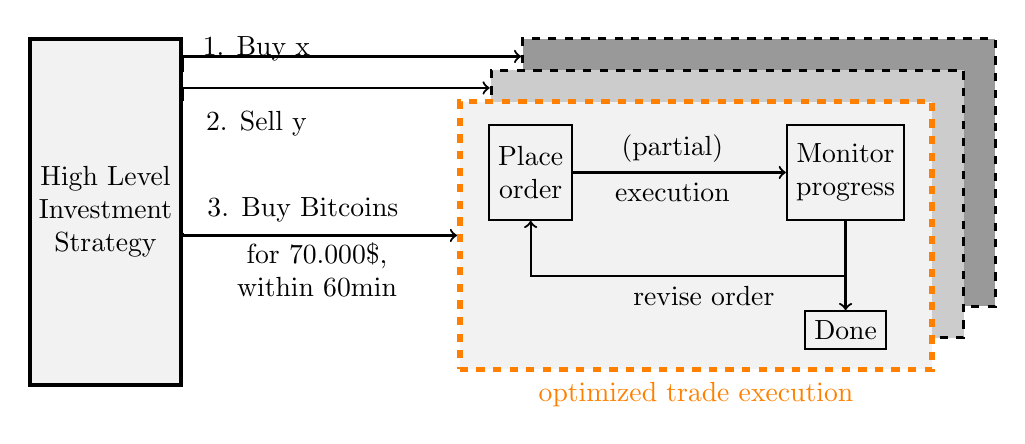
\begin{tikzpicture}[node distance = 16em, auto, thick]
    \node[draw, minimum height=4.4cm, align=center, fill=black!5, line width=0.5mm] at (0, -0.5)   (A) {High Level\\Investment\\Strategy};
    \node[draw, black, dashed, minimum height=3.4cm, minimum width=6cm, line width=0.4mm, fill=black!40] at (8.3,0) (X2) {};
    \draw[->] (A.61) node[above, xshift=2.7cm] {}  node[above, align=center, xshift=0.93cm]{1. Buy x}  |- (X2.154);
    
    \node[draw, black, dashed, minimum height=3.4cm, minimum width=6cm, line width=0.4mm, fill=black!20] at (7.9,-0.4) (X1) {};
    \draw[->] (A.55.9) node[above, xshift=2.7cm] {}  node[below, align=center, xshift=0.93cm]{2. Sell y} |- (X1.154);

    \node[draw, orange, dashed, minimum height=3.4cm, minimum width=6cm, line width=0.7mm, fill=black!5, label={below, orange: optimized trade execution}] at (7.5,-0.8) (X) {}; 

    \node[draw, minimum height=1.2cm, align=center] at (5.4, 0)   (B) {Place\\order};
    \node[draw, minimum height=1.2cm, align=center] at (9.4, 0)   (C) {Monitor\\progress};
    \node[draw, align=center] at (9.4, -2)   (D) {Done};
    
    \draw[->] (A.-15) node[above, xshift=1.52cm] {3. Buy Bitcoins}  node[below, align=center, xshift=1.7cm]{for $70.000\$$,\\within 60min} |- (X);
    \draw[->] (C.south) node[below, xshift=-1.8cm, yshift=-0.7cm] {revise order}  -- ++(-0,0) -- ++(0,-0.7) -| (B);
    \draw[->] (C.south)  -- (D);
    \draw[->] (B) node[above, xshift=1.8cm] {(partial)} node[below, xshift=1.8cm] {execution}  -- (C);

\end{tikzpicture}
	\caption{Optimized Trade Execution.}
	\label{fig:optimizedtradeexecution}
\end{figure}


In its simplest form, the problem of optimized trade execution is defined by a particular financial instrument (here: Bitcoins), which must be bought or sold within a fixed time horizon, while minimizing the expenditure (share price) for doing so.\\

This problem constitutes an ideal playground for reinforcement learning approaches, which aim to learn optimal behavior based on observed states. Regularly monitoring trade progress and market situations, reinforcement learning agents hold the potential to automatically unwind large orders over time in an advantageous way.\\

The scope of this thesis is to examine and improve the reinforcement learning approach proposed by Nevmyvaka \etal\cite{Nevmyvaka:2006}. While the authors derived valuable strategies from a discretized state space in a brute force manner, a novel forward learning algorithm is proposed, which samples from a continuous state space and outperforms the foremost algorithm. As reinforcement learning requires interacting with an environment, a trading simulation framework is implemented. The accrued \acf{OTS} provides a full-featured reinforcement learning environment, that simulates the execution of orders on historic data and returns vital feedback to steer the agent towards optimal decisions.\\

While most research is performed on traditional stock markets with expensive, proprietary data sources, this was simply out of budget for this work. Instead, the relatively young market of bitcoin trading is assessed, as it offers inexpensive access to real-time prices through publicly retrievable interfaces. Snapshots of the current market situations are retrieved on a low-resolution, minute-scale basis from the open bitcoin exchange platform Poloniex\footnote{\url{http://www.poloniex.com}}. Consequently, the usability of the retrieved dataset is analyzed.



\section{Related Work}
\label{sec:relatedwork}
bla



\section{Contributions}
\label{sec:contributions}
The following contributions to the problem of optimized trade execution have been made by this work:
\begin{itemize}
\item With the \ac{OTS}, a full-featured reinforcement learning environment for the simulation of trade execution is presented. It simulates the execution of orders on historic orderbook data and returns vital feedback to steer reinforcement learning agents towards optimal decisions.

\item An existing reinforcement learning approach, deriving valuable strategies from a discretized state space in a brute force manner, has been examined and could be improved in detail. As an example, the proposed backward-sampling method neglected the agents own impact on the market situation. It was found, that the agents cost reducing capabilities may be further improved, if this impact is incorporated properly.

\item A novel reinforcement learning approach is presented, that applies growing batch reinforcement learning on the problem of optimal trade execution. The proposed forward-sampling method samples from a more realistic, continuous state space and outperforms the foremost algorithm.

\end{itemize}

\section{Outline of Contents}
\label{sec:outline}
The remainder of this thesis is structured as follows:\\

\Cref{chap:background} gives a general introduction into the vocabulary of financial computing and the machine learning techniques employed, \Cref{chap:simulator} describes the \acl{OTS}, that provides a full-featured reinforcement learning environment. \Cref{chap:reinforcementlearning} describes and discusses both reinforcement learning approaches, \ie the original brute-force method and the novel forward learning method. \Cref{chap:orderbookagents} evaluates the performance of several trading agents emerged and \Cref{chap:conclusion} closes with a conclusion and discussion.


\cleardoublepage{}